
\chapter{Аналитический раздел}
\label{cha:analysis}

\section{Описание предметной области}

Под деревом синтаксического анализа понимается набор хранимых 
в памяти взаимосвязанных между собой типов. 
Дерево синтаксического анализа может быть создано из строки SQL запроса,
как будет показано на примере того, как postgresql выполняет запрос и какие 
структуры для этого он создает в памяти. 

\section{Анализ существующих программных решений}

\subsection{SAS Data Integration Studio}

\textit{SAS Data Integration Studio \cite{bib2}} - это инструмент визуального дизайна. 
Он создает, реализует и управляет процессами интеграции данных независимо от источников данных, приложений или платформ.

Его многопользовательская среда обеспечивает совместную работу над корпоративными проектами.
Создание и управление данными и метаданными улучшаются за счет обширного анализа воздействия потенциальных изменений, внесенных во все процессы интеграции данных.

Его встроенный редактор jobs editor позволяет создавать задачи.
На рисунке \ref{analysis:sas_create_job} продемонстрировано создание задачи.

\begin{figure}[ht!]
	\centering{
		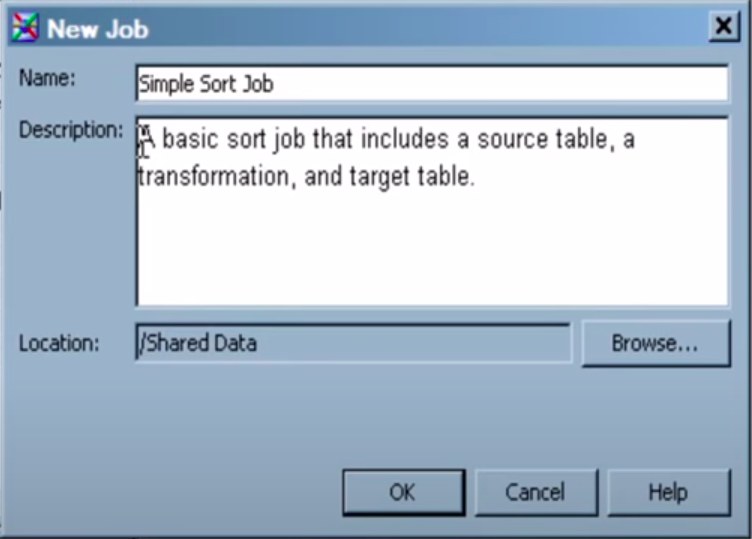
\includegraphics[width=0.95\textwidth]{img/sas_job.png}
		\caption{Демонстрация создания задачи во встроенном редакторе jobs editor программного обеспечения SAS Data Integration Studio}
		\label{analysis:sas_create_job}}
\end{figure}

После создания задачи открывается холст на котором возможно располагать графические примитивы, которые впоследствии 
будут преобразованы в запрос. % преобразования над данными.
Возможные преобразования представлены на рисунке \ref{analysis:sas_job_transform_data}. 
% Все представленные преобразования можно располагать на холсте. 
При расположении на холсте каждое преобразование превращается в графический 
примитив с данными о выполняемом преобразовании.
На рисунке \ref{analysis:sas_simple_job_example} продемонстрирована созданная задача.

\begin{figure}[ht!]
	\centering{
		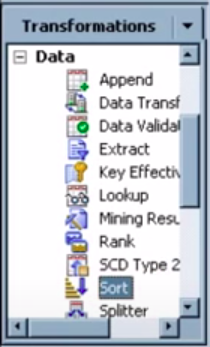
\includegraphics[width=0.4\textwidth]{img/sas_job3.png}
		\caption{Демонстрация панели трансформации во встроенном редакторе jobs editor программного обеспечения SAS Data Integration Studio}
		\label{analysis:sas_job_transform_data}}
\end{figure}

\begin{figure}[ht!]
	\centering{
		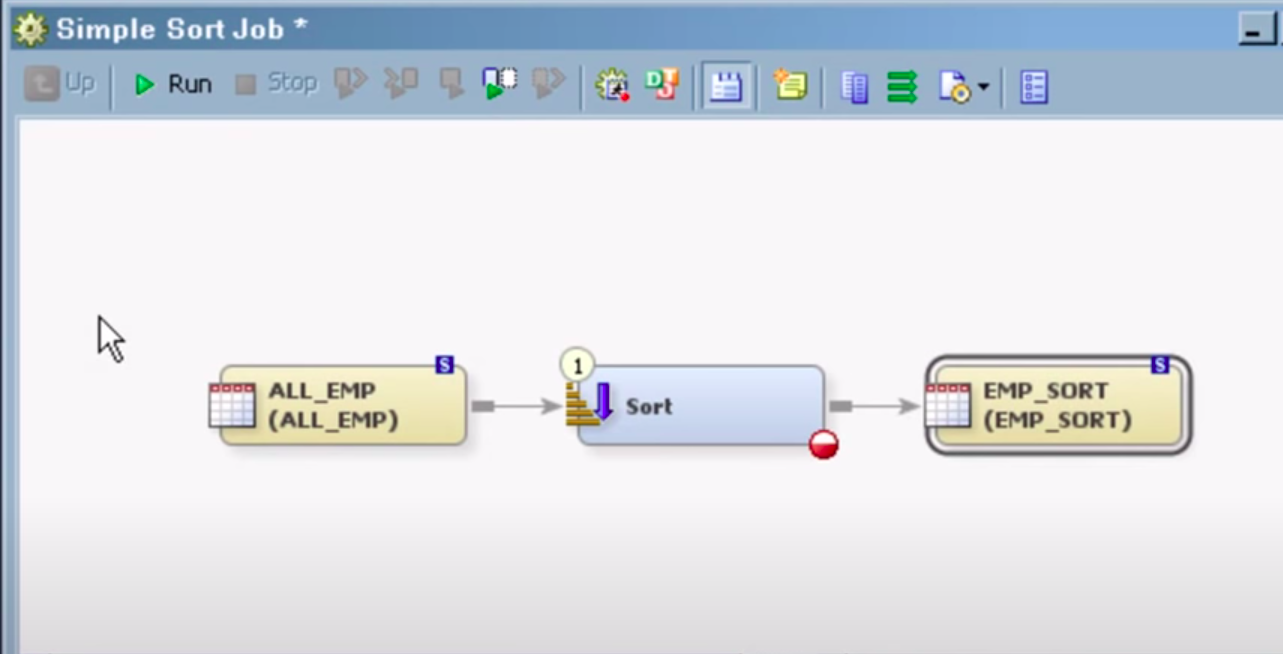
\includegraphics[width=0.95\textwidth]{img/sas_job2.png}
		\caption{Демонстрация созданной задачи во встроенном редакторе jobs editor программного обеспечения SAS Data Integration Studio}
		\label{analysis:sas_simple_job_example}}
\end{figure}

\newpage

\subsection{Informatica PowerCenter}

\textit{Informatica PowerCenter \cite{bib3}} - платформа интеграции данных, основанная на 
работе со структурами данных в визуальной среде. 
Данная платформа предоставляет возможность работать со структурами данных 
без написания программного кода, что позваоляет не только ускорить получение данных бизнесом,
но и облегчить взаимодействие с данными пользователям. 

На рисунке \ref{analysis:informatica_edit_transf} показано окно изменения данных. 
На рисунке \ref{analysis:informatica_canvas} показан холст, на котором расположены графические 
элементы, связанные между собой. 

\begin{figure}[ht!]
	\centering{
		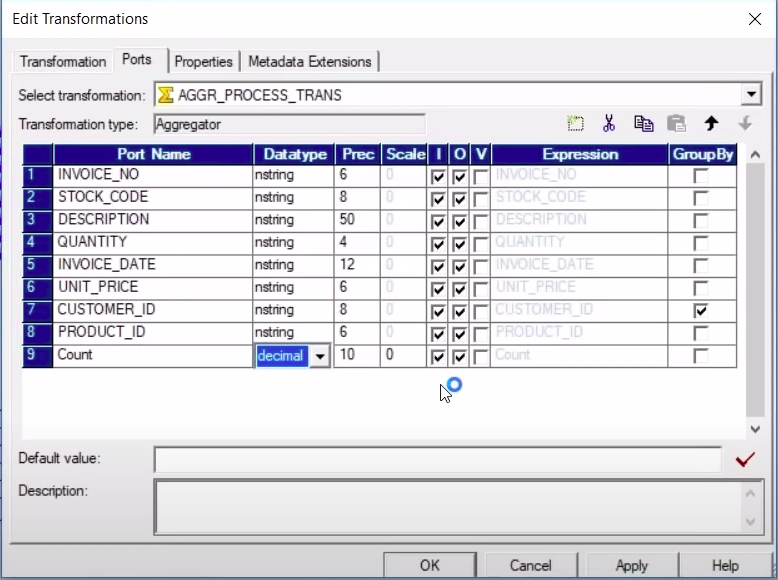
\includegraphics[width=0.95\textwidth]{img/informatica1.png}
		\caption{Окно изменения данных в платформе Informatica PowerCenter}
		\label{analysis:informatica_edit_transf}}
\end{figure}

\begin{figure}[ht!]
	\centering{
		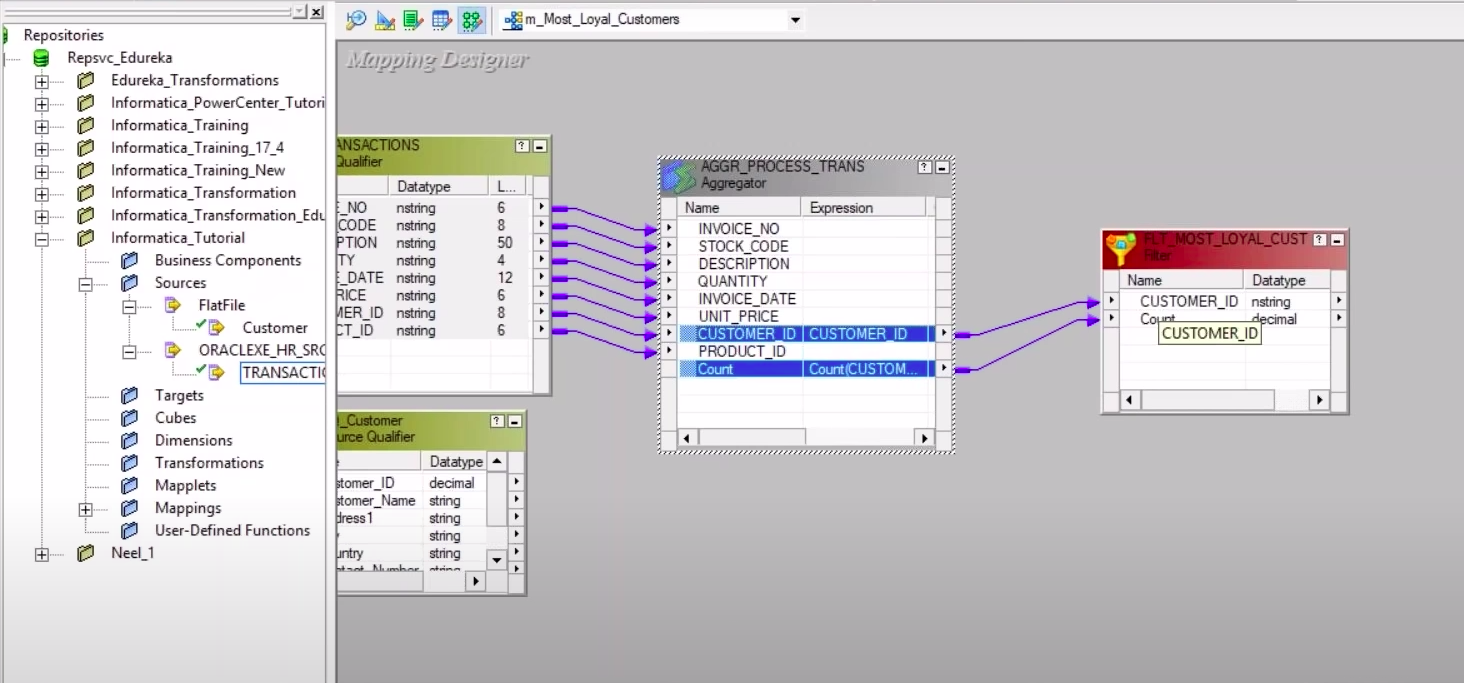
\includegraphics[width=0.95\textwidth]{img/informatica2.png}
		\caption{Холст в платформе Informatica PowerCenter}
		\label{analysis:informatica_canvas}}
\end{figure}

\newpage

\subsection{Apache NiFi}

\textit{Apache NiFi \cite{bib4}} - это программный проект от Apache Software Foundation, % предназначенный для обработки информации, 
предоставляющий возможности управления потоками 
данных из разнообразных источников в режиме реального времени с использованием графического интерфейса.
В NiFi используется веб-интерфейс для создания потоков данных.
На рисунке \ref{analysis:nifi_example} показан холст, на котором создан поток данных.

\begin{figure}[ht!]
	\centering{
		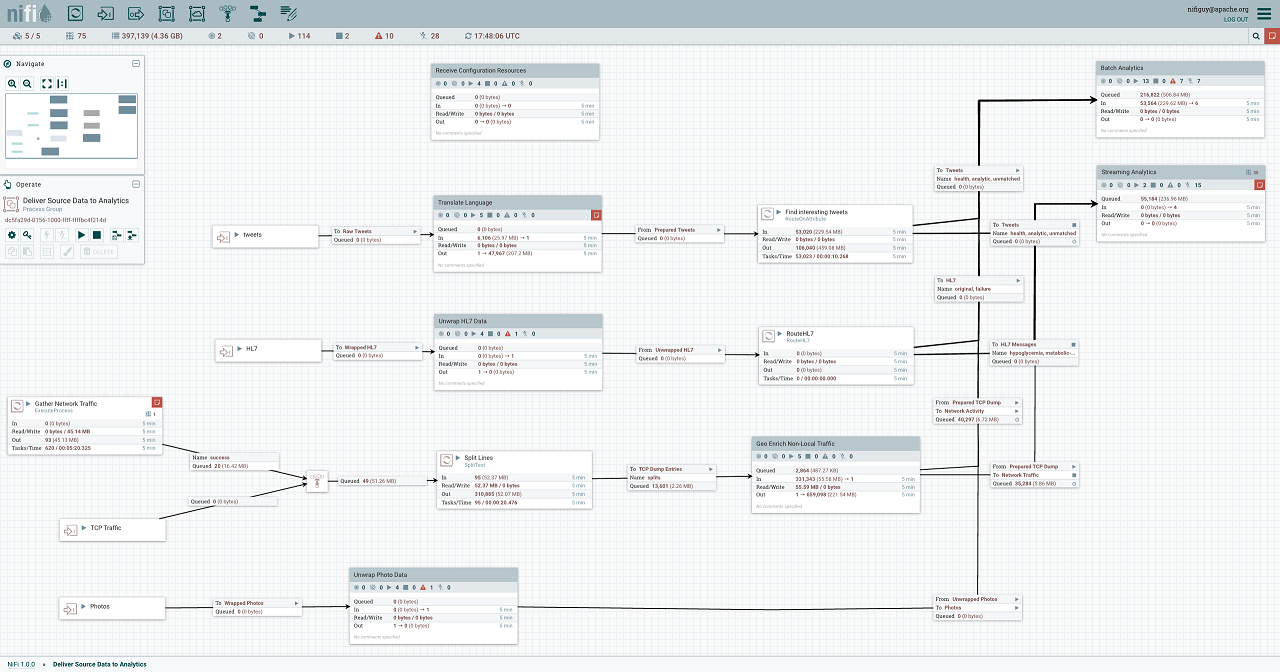
\includegraphics[width=0.95\textwidth]{img/nifi_example.png}
		\caption{Пример потока данных в программном продукте Apache NiFi}
		\label{analysis:nifi_example}}
\end{figure}

\section{План выполнения запроса postgresql}

Postgresql получает на вход набор SQL команд и обрабатывает каждую команду команду в четыре шага.

\begin{enumerate}
	\item Синтаксический анализ SQL запроса и последующее создание дерева синтаксического анализа.
	\item Оптимизация запроса.
	\item Создание плана.
	\item Выполнение.
\end{enumerate}

В postgresql функция exec\_simple\_query выполняет представленные шаги.
Рассмотрим более подробно данные шаги.

\subsection{Построение дерева синтаксического анализа}

\textit{Дерево синтаксического анализа} - набор хранимых в памяти взаимосвязанных типов. 
В случаи postgresql этот набор хранимых структур данных языка C \cite{bib1}.

С помощью синтаксического анализа postgresql конвертирует SQL запрос во 
внутреннюю структуру данных, с которой в дальнейшем он может работать.

Postgresql использует генератор синтаксического анализа Bison \cite{bib5} для 
синтаксического анализа.

Во время процесса сборки Postgresql Bison генерирует 
код парсера на основании ряда грамматических правил. 
Данный код работает внутри postgresql, когда ему отправляются SQL команды.
Далее каждое грамматическое правило вызывается, 
когда сгенерированный парсер находит соответствующий 
паттерн или синтаксис в строке SQL и вставляет новую структуру памяти C
в дерево синтаксического анализа.

Для примера рассмотрим следующий запрос 

\begin{lstlisting}[language=SQL, label=some-code, caption=Пример sql запроса над таблицей foo]
SELECT * FROM foo where bar = 42 ORDER BY id DESC LIMIT 23;
\end{lstlisting}

Данный запрос преобразуется в следующее дерево синтаксического анализа.

\begin{lstlisting}[label=some-code, caption=Дерево синтаксического анализа для SQL запроса над таблицей foo]
(
   {SELECT 
   :distinctClause <> 
   :intoClause <> 
   :targetList (
      {RESTARGET 
      :name <> 
      :indirection <> 
      :val 
         {COLUMNREF 
         :fields (
            {A_STAR
            }
         )
         :location 7
         }
      :location 7
      }
   )
   :fromClause (
      {RANGEVAR 
      :schemaname <> 
      :relname foo 
      :inhOpt 2 
      :relpersistence p 
      :alias <> 
      :location 14
      }
   )
   :whereClause 
      {AEXPR  
      :name ("=")
      :lexpr 
         {COLUMNREF 
         :fields ("bar")
         :location 24
         }
      :rexpr 
         {A_CONST 
         :val 42 
         :location 30
         }
      :location 28
      }
   :groupClause <> 
   :havingClause <> 
   :windowClause <> 
   :valuesLists <> 
   :sortClause (
      {SORTBY 
      :node 
         {COLUMNREF 
         :fields ("id")
         :location 42
         }
      :sortby_dir 2 
      :sortby_nulls 0 
      :useOp <> 
      :location -1
      }
   )
   :limitOffset <> 
   :limitCount 
      {A_CONST 
      :val 23 
      :location 56
      }
   :lockingClause <> 
   :withClause <> 
   :op 0 
   :all false 
   :larg <> 
   :rarg <>
   }
)
\end{lstlisting}

Рассмотрим еще один запрос (листинг 1.3). 
На рисунке \ref{analysis:pg_step_1_tree} проиллюстрировано дерево синтаксического анализа, 
которое создал postgresql из запроса представленного в листинге 1.3.

\begin{lstlisting}[language=SQL, label=some-code, caption=Пример SQL запроса над таблицей users]
SELECT * FROM users
WHERE name = 'Capian Nemo'
ORDER BY id ASC
LIMIT 1;
\end{lstlisting}

\begin{figure}[ht!]
	\centering{
		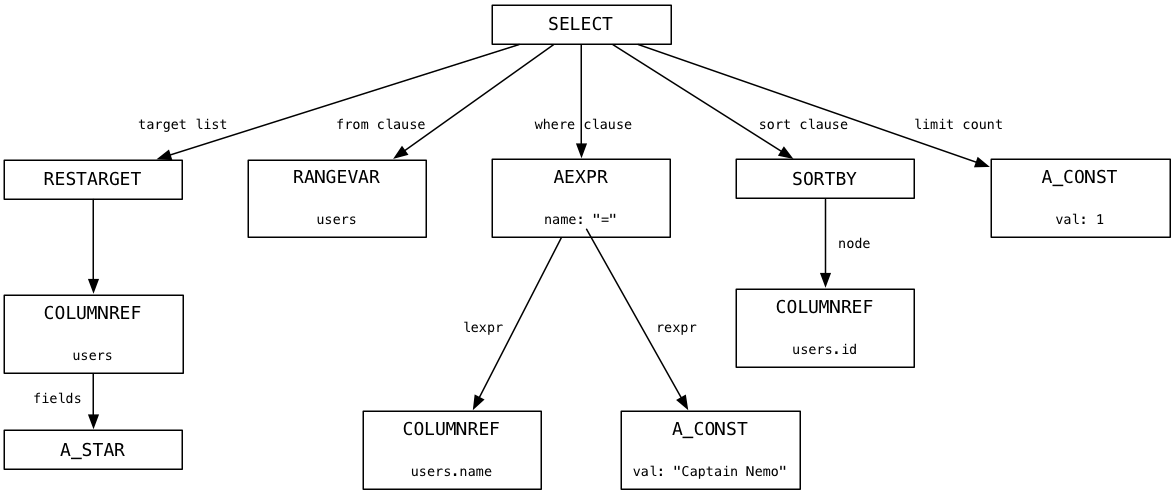
\includegraphics[width=1\textwidth]{img/pg_step_1_tree.png}
		\caption{Дерево синтаксического анализа для SQL запроса из таблицы users}
		\label{analysis:pg_step_1_tree}}
\end{figure}

\subsection{Оптимизация}

После того, как postgresql создал дерево синтаксического анализа из переданного ему SQL запроса,
он преобразовывает его, применяя оптимизации, в другое дерево, используя другой набор узлов.
Полученное дерево называется деревом запроса.
Процесс оптимизации применяет ряд сложных алгоритмов и эвристик в 
попытке оптимизировать и упростить SQL запрос.

Для приведенного выше запроса (листинг 1.3) postgresql преобразовал дерево 
синтаксического анализа в дерево,
представленное на рисунке \ref{analysis:pg_step_2_tree}.

\begin{figure}[ht!]
	\centering{
		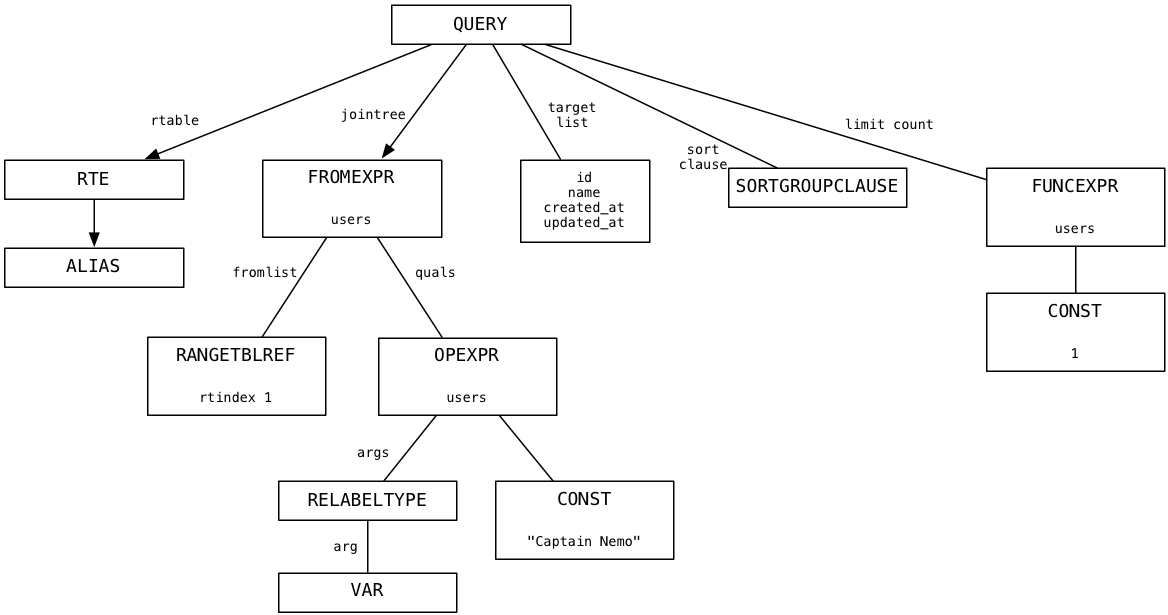
\includegraphics[width=1\textwidth]{img/pg_step_2_tree.png}
		\caption{Дерево запроса для SQL запроса из таблицы users}
		\label{analysis:pg_step_2_tree}}
\end{figure}

\subsection{Создание плана}

Перед тем, как начать выполнять запрос, postgresql создает план.
Данный процесс включает в себя создание третьего дерева узлов, 
которые представляют собой список инструкций для postgresql.
Для приведенного выше запроса (листинг 1.3) postgresql построил 
дерево плана, которое показано на рисунке \ref{analysis:pg_step_3_tree}.

\begin{figure}[ht!]
	\centering{
		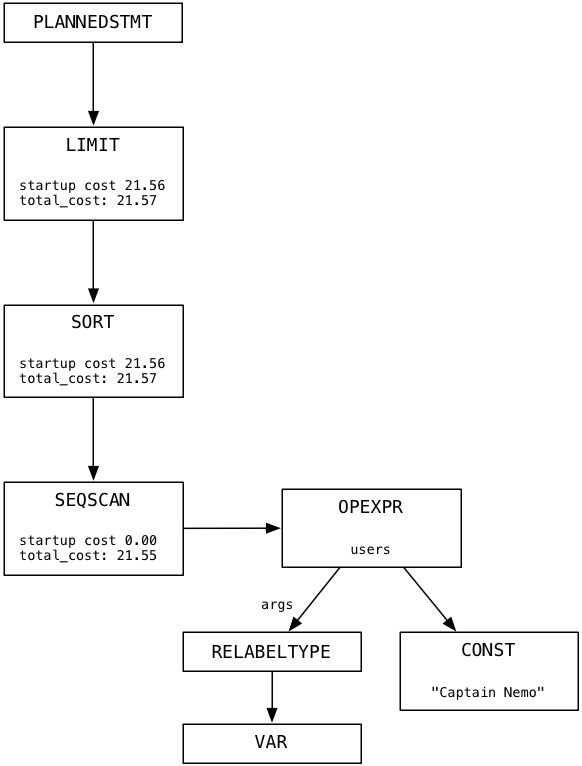
\includegraphics[width=0.6\textwidth]{img/pg_step_3_tree.png}
		\caption{План для SQL запроса из таблицы users}
		\label{analysis:pg_step_3_tree}}
\end{figure}

\subsection{Выполнение}

На шаге выполнения запроса postgresql уже преобразовал переданный ему в с самом начале 
SQL запрос в синтаксическое дерево анализа, оптимизировал и построил план запроса.
postgresql имеет план, которому будет следовать, чтобы получить результат.
postgresql для каждого нижележащего узла берет данные и возвращает их 
в качестве исходных данных для узла выше. 
Таким образом данный итеративный процесс повторяется,
пока что не будут получены данные из самого верхнего узла.
Это и будет являться результатом SQL запроса.

\section{Грамматика}


